% !TeX root = ../main.tex
% Add the above to each chapter to make compiling the PDF easier in some editors.

\chapter{Solving Laplacian Linear Systems}

We have seen by now that many problems can be reduced to solving a Laplacian linear system $\mL\vx = \vd$ where $\vd \in \im{L} = \compl{(\ker{\mL})}$. Recall that we can obtain a Cholesky decomposition $\mL = \mCalL\trans{\mCalL}$ where $\mCalL$ is lower-triangular and positive semi-definite. If $\mL$ (and therefore $\mCalL$) were invertible, then we have seen that the linear system can be solved in time $\LandauO{\nnz{\mCalL}}$. However, we know that $\mL$ is not invertible as $\ker{\mL} \neq \{\vZero\}$. It turns out that we can still use of a Cholesky decomposition in solving Laplacian linear systems because we have a simple characterization of the kernel of $\mL$. This we will discuss first, then we discuss how to efficiently compute the Cholesky decomposition.

\begin{thm}
We can solve the linear system $\mL\vx = \vd$ where $\vd \perp \vOne$ in time $\LandauO{n^3}$ by first computing a Cholesky decomposition of $\mL$ using Gaussian elimination and then applying the pseudoinverse $\pinv{\mL}$ to $\vd$.
\end{thm}

Finally, we will see that we can find approximate solutions in almost linear time.

\section{Dealing with pseudoinverses}

A natural approach is to characterize the pseudoinverse $\pinv{\mL}$ in terms of the lower triangular matrix $\mCalL$.

\begin{lem}
Given a factorization $\mL = \mCalL\trans{\mCalL}$ where $\mCalL$ is lower triangular and all diagonal entries are strictly non-zero except that $\mCalL(n,n) = 0$, we can apply $\pinv{\mL}$ in time $\LandauO{n}$.
\end{lem}
\begin{proof} Consider the matrix $\hat{\mCalL}$, which is identical to $\mCalL$ except that $\hat{\mCalL}(n,n) = 1$. Let $\mCalD$ be the diagonal matrix with $\mCalD(i,i) = 1$ for $i < n$ and $\mCalD(n,n) = 0$. Then, $\mCalL\trans{\mCalL} = \hat{\mCalL}\mCalD\trans{\hat{\mCalL}}$ and $\hat{\mCalL}$ is invertible. By \cref{clm:pinv_calculation}, we have \begin{align*}
    \pinv{\mL} = \mPi_\mL \inv{(\trans{\hat{\mCalL}})} \pinv{\mCalD} \inv{\hat{\mCalL}} \mPi_\mL,
\end{align*} where $\mPi_\mL$ is the orthogonal projection to the kernel of $\mL$. Note that $\mPi_\mL = \mI - \frac{1}{n}\vOne\trans{\vOne}$, as this satisfies $\mPi_\mL\vv = \vv$ for $\vv \perp \vOne$ and $\mPi_\mL\vv = \vZero$ for $\vv \in \vspan\{\vOne\}$. We also have $\pinv{\mCalD} = \mCalD$.

Finally, observe that $\mPi_\mL$ and $\mCalD$ can be applied in time $\LandauO{n}$; and by \cref{lem:solve_triangular_linear_system}, we can apply $\inv{\hat{\mCalL}}$ and $\inv{(\trans{\hat{\mCalL}})}$ in time $\LandauO{\nnz{\mCalL}}$.
\end{proof}

\section{Computing the Cholesky Decomposition}

\begin{thm}[Cholesky decomposition on graph Laplacians] Using Gaussian elimination, we can compute in $\LandauO{n^3}$ time a factorization $\mL~=~\mCalL\trans{\mCalL}$, where $\mCalL$ is lower triangular and has positive diagonal entries except that $\mCalL(n,n) = 0$.
\end{thm}
\begin{proof}
Let $\mL^{(0)} \defeq \mL$. For $i \in [n-1]$, we define, \begin{align*}
    \vl_i &\defeq \frac{1}{\sqrt{\mL^{(i-1)}(i,i)}}\mL^{(i-1)}(:,i) \quad\text{and} \\
    \mL^{(i)} &\defeq \mL^{(i-1)} - \vl_i \trans{\vl_i}.
\end{align*}

\begin{clm}\label{clm:cholesky_decomp_intermediate_laplacians}
Fix some $i < n$. Let $\sU \defeq \{i+1, \dots, n\}$. Then, $\mL^{(i)}(i,j) = 0$ if $i \not\in \sU$ or $j \not\in \sU$; and $\mL^{(i)}$ is a graph Laplacian matrix of a connected graph on the vertex set $\sU$.
\end{clm}

It follows that $\mL^{(n-1)} = \mZero_{n \times n}$ because the only graph on a single vertex is the empty graph. From this, we have that $\mL = \sum_{i=1}^{n-1} \vl_i \trans{\vl_i}$ provided that $\vl_i$ is well-defined, i.e., $\mL^{(i-1)}(i,i) \neq 0$ for all $i < n$. But this follows immediately from the claim, as the diagonal of the Laplacian matrix of a connected graph on more than one vertex must be strictly positive (as the degrees must be non-zero).

In each iteration, we compute $\mL^{(i)}$ in time $\LandauO{n^2}$ and we proceed for $\LandauO{n}$ iterations.
\end{proof}

\begin{proof}[Proof sketch of \cref{clm:cholesky_decomp_intermediate_laplacians}] We focus on the first elimination, the remaining are similar. We write, \begin{align*}
    \mL^{(0)} = \mL \eqdef \begin{bmatrix}
        w & -\trans{\va} \\
        -\va & \diag(\va) + \mL_{-1} \\
    \end{bmatrix},
\end{align*} where $\mL_{-1}$ is defined to make the equality work. We have that, \begin{align*}
    \vl_1 = \frac{1}{\sqrt{w}}\begin{bmatrix}
        w \\
        -\va \\
    \end{bmatrix} \quad\text{and}\quad \vl_1 \trans{\vl_1} = \begin{bmatrix}
        w & -\trans{\va} \\
        -\va & \frac{1}{w}\va\trans{\va} \\
    \end{bmatrix}
\end{align*} Therefore, \begin{align*}
    \mL^{(1)} = \mL^{(0)} - \vl_1 \trans{\vl_1} = \begin{bmatrix}
        0 & \trans{\vZero} \\
        \vZero & \mS^{(0)} \\
    \end{bmatrix},
\end{align*} where $\mS^{(1)} \defeq \mL_{+1} + \mL_{-1}$ and $\mL_{+1} \defeq \diag(\va) - \frac{1}{w}\va\trans{\va}$. $\mS^{(1)}$ is also called the \emph{Schur complement}\index{Schur complement}. It remains to show that $\mS^{(1)}$ is the Laplacian matrix of a connected graph on the vertex set $\{2, \dots, n\}$.

\begin{marginfigure}
TBD
% \centering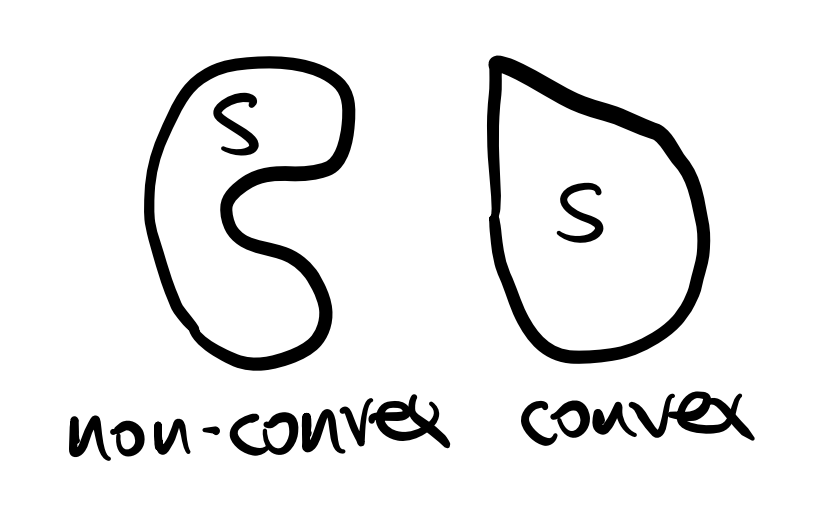
\includegraphics[width=4cm]{notes/figures/convex_set.png}
\caption{$\mS^{(1)}$ is the Laplacian matrix of the graph, where the first vertex was removed and all of its neighbors are made to be in a clique.}
\end{marginfigure}

Observe that the sum of two Laplacian matrices is a again a graph Laplacian. Therefore, $\mL_{-1}$ is a graph Laplacian by definition. It is easy to check that by the characterization of \cref{exc:graph_laplacian_characterization}, $\mL_{+1}$ also is a graph Laplacian, which represents a clique formed by the neighbors of vertex $1$. Hence, $\mS^{(1)} = \mL_{+1} + \mL_{-1}$ is a graph Laplacian.

It remains to show that the underlying graph is connected. Consider any $i,j \in \sV \setminus \{1\}$. There exists an $i$-$j$ path $P$ in the graph of $\mL$. If $P$ does not use vertex $1$, then $P$ is a path in the graph of $\mL_{-1}$. If $P$ does use vertex $1$, it does so using some edges $(u,1)$ and $(1,v)$. Replacing the two edges with the edge $(u,v)$, which appears in $\mL_{+1}$ as $\mL_{+1}(u,v) < 0$, yields a path in the graph of $\mS^{(1)}$.
\end{proof}

\section{Approximate Almost Linear-Time Solvers}

\begin{defn}[Approximate solution to linear system] We say that $\Tilde{\vx}$ is an \emph{$\epsilon$-approximate solution}\index{approximate solution to linear system} to the linear system $\mA\vx = \vb$ iff \begin{align}
    \norm{\Tilde{\vx} - \s{\vx}}_\mA^2 \leq \epsilon \norm{\s{\vx}}_\mA^2,
\end{align} where $\s{\vx}$ is a solution and $\norm{\vy}_\mA \defeq \sqrt{\trans{\vy}\mA\vy}$ denotes the \emph{Mahalanobis norm}\index{Mahalanobis norm} with respect to $\mA$.
\end{defn}

The fast algorithm has two main steps.

\begin{thm}[Approximate Cholesky decomposition on graph Laplacians] We can find $\mCalL\trans{\mCalL} \approx_{\nicefrac{1}{2}} \mL$ such that $\mCalL$ is lower triangular and $\nnz{\mCalL} = \LandauO{m \log^3 n}$, with probability at least $1 - \nicefrac{3}{n^5}$ in time $\LandauO{m \log^3 n}$.\cite{kyng2016approximate}
\end{thm}
\begin{proof}
TBD
\end{proof}

Here, the main idea is to replace the clique of the neighbors of the eliminated vertex in each round of Gaussian elimination by a sparse approximation.

\begin{thm} We can find an $\epsilon$-approximate solution $\Tilde{\vx}$ to $\mL\vx = \vd$, using an algorithm that takes $\LandauO{m \log^3 n \log(\nicefrac{1}{\epsilon})}$ time and succeeds with probability at least $1 - \nicefrac{1}{n^{10}}$.
\end{thm}
\begin{proof}
TBD
\end{proof}